\section{Chronologische Entwicklung didaktischer Simulatoren}

\TODO{Kapitel ggf. kürzen, begrenzen auf Rechnerarchitektur oder nur auf Milestones der Rechenerarchitektur eingehen}

\subsection{Mechanische Lern- \& Lehrmaschinen}

Die Entwicklung didaktischer Simulatoren lässt sich über mehrere Jahrhunderte hinweg nachzeichnen. Erste Vorläufer finden sich bereits 1588, als Agostino Remelli ein sogenanntes \textit{Leserad} konzipierte, das die parallele Nutzung mehrerer Bücher erleichtern sollte und somit als frühe mechanische Lernhilfe gelten kann \parencite{cayetano_geschichte_2022}.

Ein bedeutender Meilenstein in der Entwicklung früher Lernmaschinen wurde im Jahr 1866 durch das Patent von Halycon Skinner gesetzt. Er konstruierte ein Gerät, bei dem nach der visuellen Darstellung eines Bildes auf einem Kasten die korrekte Bezeichnung über eine Schreibmaschinentastatur eingegeben werden musste. Die Maschine erwies sich jedoch als äußerst fehleranfällig: Falsche Begriffe wurden bei korrekter Orthographie als richtig gewertet, was die Zuverlässigkeit des Systems stark einschränkte. Im Jahr 1911 griff Herbert Aiken Skinners Konzept auf und entwickelte eine verbesserte Version, die er als „Buchstabiermaschine“ präsentierte. Diese Lernvorrichtung basierte auf einem mechanischen Rahmen, in den mit Buchstaben beschriftete Karten eingesetzt wurden. Die puzzleartige Konstruktion erlaubte das Ausprobieren verschiedener Kombinationen, wobei ausschließlich die korrekte Lösung zum Erfolg führte und das „Puzzle“ vervollständigte. Bis 1936 wurden rund 700 Patente für derartige Übungsmaschinen angemeldet. Das grundsätzliche Lernkonzept hinter diesen Maschinen ist das \textit{law of effect} des amerikanischen Psychologen Edward L. Thorndike \parencite[S.~3]{niegemann_kompendium_2008}.

Bereits 1928 stellte \textbf{Sidney Leavitt Pressey} eine „Maschine für Intelligenztests“ vor, die zu den einflussreichsten Vorläufern späterer Lehrmaschinen zählt. Sie arbeitete mit Multiple-Choice-Aufgaben, wobei die Lernenden ihre Antworten über nummerierte Tasten eingaben. Ein eingebauter Zähler registrierte die Anzahl richtiger Lösungen. Bemerkenswert ist, dass Pressey darüber hinaus -- in Anlehnung an das zeitgleich entwickelte „law of effect“ -- einen Belohnungsmechanismus integrierte: Bei einer korrekten Antwort gab die Maschine eine Süßigkeit aus. Damit machte Pressey deutlich, dass psychologische Faktoren wie Motivation und Verstärkung zentrale Elemente bei der Gestaltung von Lern- und Lehrmaschinen sein können \parencites[S.~705]{benjamin_history_1988}[S.~969f]{skinner_teaching_1958}.

In den 1950er Jahren erhielten die von \textbf{Burrhus F. Skinner} und \textbf{James G. Holland} entwickelten Lehrmaschinen zunehmende Aufmerksamkeit. Diese „Skinner-Holland’schen Maschinen“ beruhten explizit auf der behavioristischen Lerntheorie und folgten dem Prinzip des programmierten Lernens: Der Stoff wurde in kleine Einheiten (\textit{Frames}) zerlegt, auf die jeweils Fragen folgten. Lernende konnten ihre Eingabe direkt mit der richtigen Lösung vergleichen und erhielten so unmittelbares Feedback \parencite[S.~970--977]{skinner_teaching_1958}. Bereits hier lassen sich die zentralen Prinzipien des programmierten Unterrichts erkennen: Die Strukturierung des Lernstoffs in kleine Schritte, die Anpassung an das individuelle Lerntempo, die aktive Beteiligung durch Antworten sowie die sofortige Rückmeldung \parencite[S.~1971]{bruillard_teaching_2020}. Diese didaktischen Grundsätze wurden in den 1960er Jahren auf den Computer übertragen und bildeten die Basis für die Entwicklung der computergestützten Instruktion.

Im Gegensatz zu den linearen Lehrprogrammen entwickelte \textbf{Norman Crowder} im Jahr 1959 das Konzept der sogenannten „verzweigten Lernprogramme“, die eine erste Form der Individualisierung im Lehr-Lernprozess ermöglichten. Diese Programme reagierten adaptiv auf die Fehler der Lernenden, indem sie unterschiedliche Lernpfade eröffneten. Charakteristisch für Crowders Ansatz sind umfangreichere Frames, die jeweils durch eine Multiple-Choice-Frage abgeschlossen werden. Bei Auswahl einer falschen Antwort erhielt der Lernende eine spezifische Rückmeldung, die auf die Art des Fehlers abgestimmt war. Anschließend führte das Programm entlang einer fehlerabhängigen Sequenz weiter, wobei zuvor behandelte Inhalte bei Bedarf erneut präsentiert wurden, sofern ein Verständnisdefizit vermutet wurde \parencites[S.~252--254]{crowder_differences_1963}[S.~9]{schonfeld_computerbasiertes_2006}. Crowders Ansatz gilt damit als wichtiger Schritt hin zu adaptiven Lernsystemen, die später in den 1960er Jahren mit dem Aufkommen computergestützter Instruktion (CAI) technisch umgesetzt werden konnten.

\subsection{Computer Assisted Instruction}

\sh{Entwicklungen in den USA}
 Ab den 1960er Jahren fanden computergestützten Instruktion (CAI – Computer Assisted Instruction) zunächst weite Verbreitung, verloren jedoch Mitte des Jahrzehnts an öffentlicher Aufmerksamkeit. Neue Impulse gingen von großangelegten US-Projekten aus, die 1971 durch die National Science Foundation initiiert wurden. Dazu zählten \textit{PLATO} (Programmed Logic for Automatic Teaching Operation) und \textit{TICCIT} (Time-shared Interactive Computer Controlled Information Television), die erstmals computerbasierte Instruktion in großem Maßstab demonstrierten \parencites[S.~7]{niegemann_kompendium_2008}[S.~69ff]{oshea_lernen_1986}.

\textit{TICCIT} ermöglichte den Lernenden eine individuelle Steuerung ihres Lernprozesses, insbesondere in den Fächern Mathematik und Englischaufsatz. Während bei vollständiger Nutzung gute Lernergebnisse erzielt wurden, war die Abbruchquote deutlich höher als im Präsenzunterricht. Als Ursachen gelten mangelnde Selbstorganisation der Lernenden sowie die geringe Akzeptanz durch Lehrende, was letztlich zum Scheitern des Projekts beitrug. Dennoch gilt TICCIT als technologisch bedeutsamer Fortschritt \parencites[S.~71]{oshea_lernen_1986}[S.~13]{schonfeld_computerbasiertes_2006}.

\textit{PLATO} bot im Vergleich dazu eine weiterentwickelte Form computerunterstützter Instruktion, die vor allem durch interaktive Simulationen am Bildschirm überzeugte. Zwar waren die Lernergebnisse ähnlich wie bei TICCIT, jedoch war die Abbruchquote geringer, und viele Lernende nutzten das System freiwillig über die Kurszeiten hinaus. PLATO gilt daher als besonders motivationsförderndes Lernsystem mit hoher Nutzerbindung \parencites[S.~75f]{oshea_lernen_1986}[S.~14]{schonfeld_computerbasiertes_2006}.

\sh{Entwicklungen in Deutschland und Europa}
Parallel zu den großangelegten US-Projekten entstanden in Deutschland ab 1964 verschiedene Lehrmaschinen, darunter der \textit{Robbimat 0}, der \textit{Geromat III} und der \textit{Bakkalaureus}, die vor allem für die Gruppenschulung eingesetzt wurden. Weitere Forschungsinitiativen bildeten sich mit dem Bildungstechnologischen Zentrum in Wiesbaden sowie dem „Forschungs- und Entwicklungszentrum für objektivierte Lehr- und Lernverfahren“ (FEoLL) in Paderborn. In Berlin wurde zudem das Projekt \textit{ALCU} (Algorithmierung von Lehrprogrammen für computergesteuerten Unterricht) erprobt, das die systematische Erstellung von Lehrprogrammen für den computergestützten Unterricht zum Ziel hatte \parencites[S.~10]{niegemann_kompendium_2008}[S.~11]{schonfeld_computerbasiertes_2006}.

In den frühen 1970er Jahren entstanden an der Universität Freiburg Programme wie \textit{PFLABE}, das Biologiestudierenden Wissen als Ersatz für Praktika vermitteln sollte, sowie \textit{ZOPRAM}, das darauf abzielte, Vorwissensunterschiede zwischen Studierenden auszugleichen. Die Begleituntersuchungen zeigten, dass der Lernerfolg von \textit{PFLABE}-Nutzenden nicht über dem der Vergleichsgruppe im Praktikum lag, jedoch der Zeitaufwand für das Lernen mit dem Programm deutlich geringer war. Gleichzeitig wurden auch Simulationsprogramme entwickelt, die praxisnahes Lernen in experimentellen Szenarien unterstützen sollten \parencite[S.~11]{niegemann_kompendium_2008}.

Nach einer Phase des Rückgangs in den späten 1970er und frühen 1980er Jahren erlebte das computergestützte Lernen Mitte der 1980er Jahre eine Renaissance, insbesondere durch methodisch anspruchsvollere Programme wie \textit{KAVIS}/\textit{KAVIS II} für den Biologieunterricht. Ab Mitte der 1990er Jahre gewann computergestütztes Lernen durch die zunehmende Verfügbarkeit von Personal Computern und den Aufschwung des World Wide Webs (siehe dazu Abb.~\ref{fig:rechner_internet}und Abb.~\ref{fig:internetnutzer} ) erneut erheblich an Bedeutung und führte schließlich zur Etablierung des Begriffs \enquote{E-Learning} \parencite[S.~11]{niegemann_kompendium_2008}.

\begin{figure}[h!]
    \centering
    \begin{subfigure}[b]{0.48\textwidth}
        \centering
        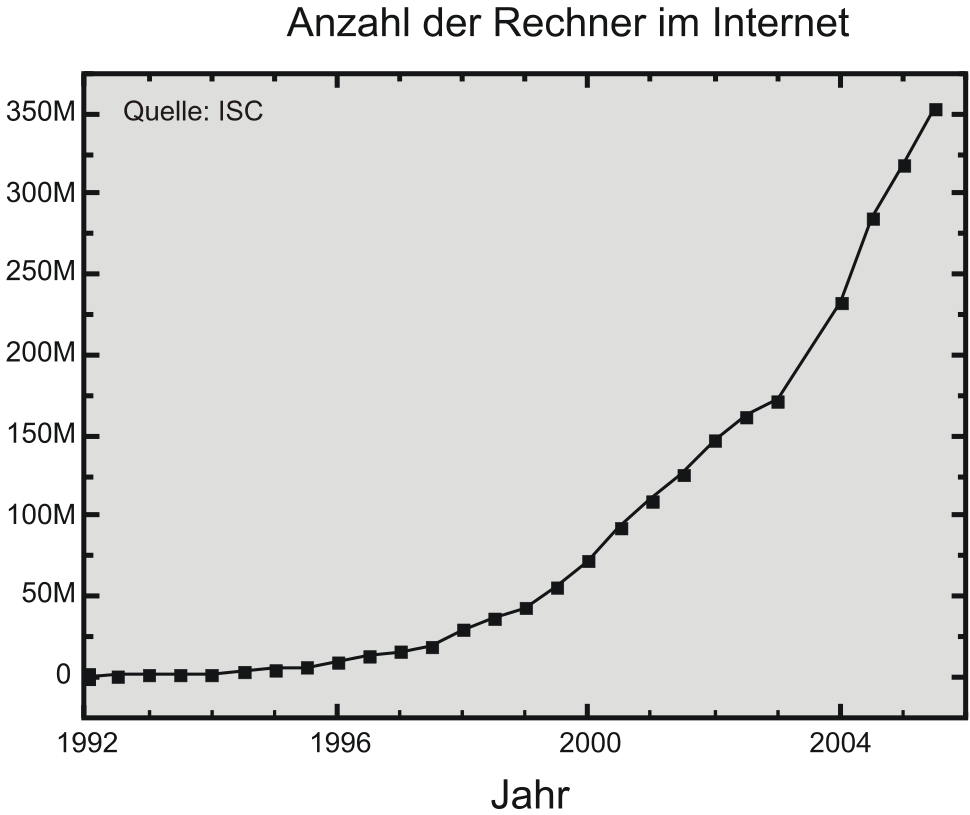
\includegraphics[width=\textwidth]{img/Anzahl_Rechner_im_Internet-2004.png}
        \caption{Anzahl der Rechner im Internet}
        \label{fig:rechner_internet}
		\cite{internet_systems_consortium_internet_2005}
    \end{subfigure}
    \hfill
    \begin{subfigure}[b]{0.48\textwidth}
        \centering
        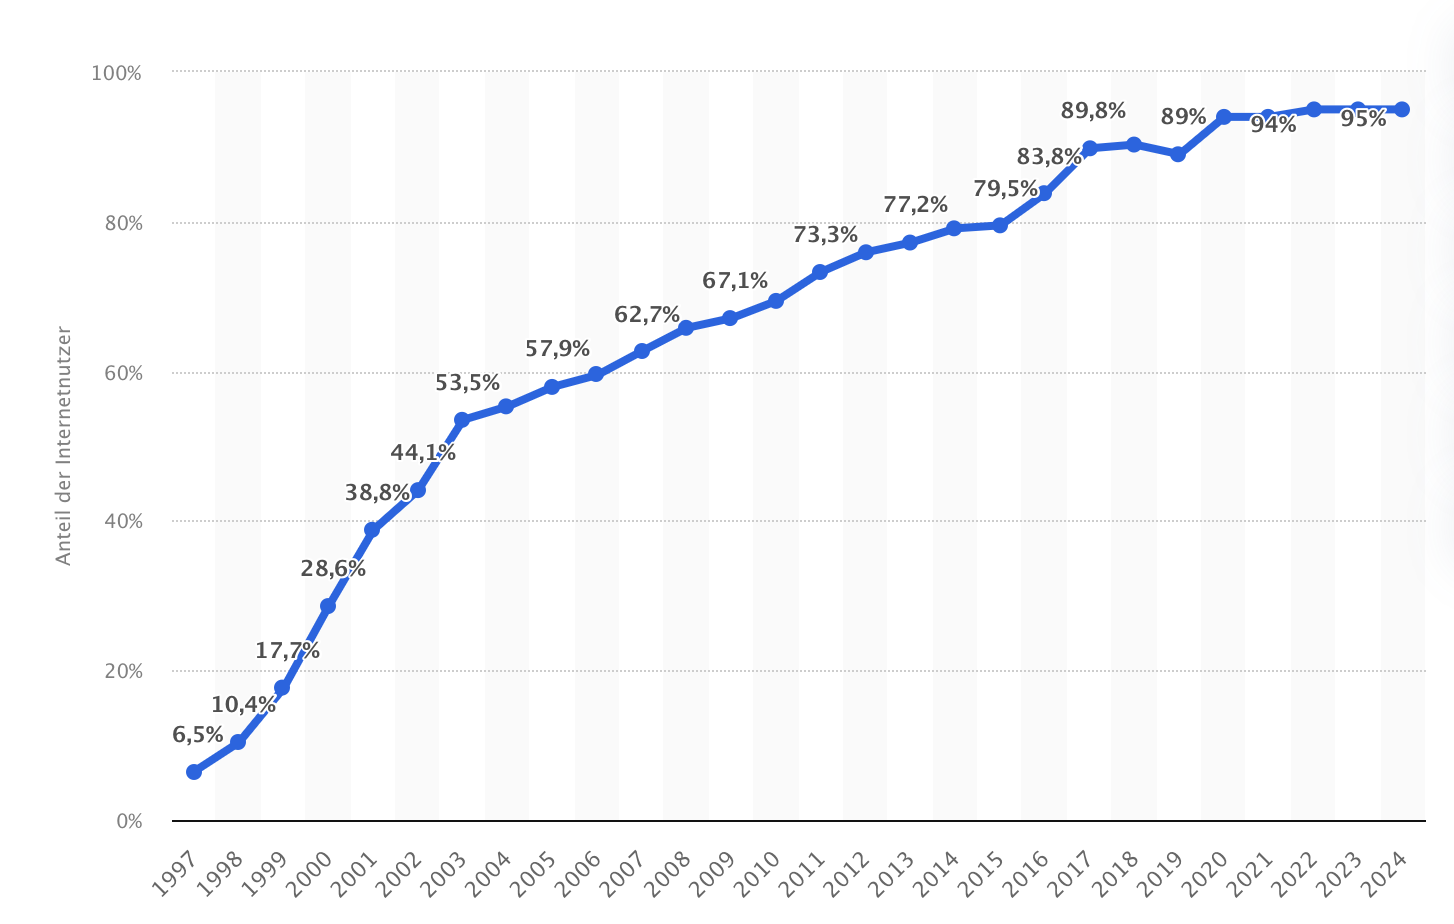
\includegraphics[width=\textwidth]{img/Anzahl_Internetnutzer-2024.png}
        \caption{Anteil der Internetnutzer in Deutschland in den Jahren 1997 bis 2024}
        \label{fig:internetnutzer}
		\cite{statista_anteil_2024}
    \end{subfigure}
    \caption{Aufschwung des World Wide Webs}
    \label{fig:www}
\end{figure}

\subsection{Web~2.0 \& E-Learning}

Mit der Initiative „Schulen ans Netz“ \cite{schulen_ans_netz_ev_schulen_nodate} wurde im Jahr 2001 die flächendeckende Internetanbindung deutscher Schulen erreicht \cite{kopcke_internet_2016}. In den 2000er Jahren entstanden zahlreiche vom Bundesministerium für Bildung und Forschung (BMBF) geförderte Projekte, die sich speziell mit der Visualisierung und Simulation in der Informatik-Didaktik befassten. Dazu zählen unter anderem \textit{SIMBA} (Schlüsselkonzepte der Informatik in multimedialen Bausteinen)\footnote{Das BMBF-Verbundprojekt SIMBA und darin das Teilprojekt Rechnernetze basieren auf netzbasiertem Lernmaterial wie Hypertexten, Grafiken und Animationen \parencite[S.~75]{magenheim_blended_2003}.}, \textit{MuSofT} (Multimedia in der Softwaretechnik) \footnote{Ziel des MuSofT-Projekts war es, für die Software-Engineering-Ausbildung multimediale Materialien bereitzustellen und ein Konzept für Blended Learning zu entwickeln \parencite[S.~73]{magenheim_blended_2003}.}, \textit{RaVi} (Rechnerarchitektur-Visualisierung) \footnote{Das RaVi-Projekt machte dynamische Abläufe in Rechnersystemen anschaulich und berücksichtigte dabei gezielt frauenspezifische Lerninteressen \parencite[S.~20]{marwedel_interaktive_2003}.} sowie die Wissenswerkstatt Rechensysteme (\textit{WWR}) \footnote{WWR ist ein Baukastensystem aus multimedialen, skalier- und rekombinierbaren Lehr- und Lernmodulen \parencite[S.~1]{kornelsen_inhalte_2004}.}. Alle diese Projekte verfolgten das Ziel, komplexe Vorgänge in Rechnersystemen durch interaktive und multimediale Simulationen für Lernende erfahrbar zu machen.

Ab etwa 2002 lässt sich eine Veränderung in der Entwicklung digitaler Lernmedien beobachten. Niegemann arbeitet in seinem Lehrbuch auf dem Jahr 2009 heraus, dass die Euphorie für E-Learning seit 2002 etwas abzuflachen schien, da viele Erwartungen nicht erfüllt wurden. Allerdings habe sich E-Learning als Lehr- und Lernform dennoch etabliert (die Diskussion zum E-Learning wird im Kapitel~\ref{diskussion_elearning} nochmal aufgegriffen) \parencite[S.~14]{niegemann_kompendium_2008}.

Mit der Ausweitung des \textbf{Web~2.0} \footnote{In einem Artikel aus September 2005 listet Tim O'Reilly die nachfolgenden Kernkompetenzen des Web~2.0 auf: \textit{„Services, not packaged Software; Architecture of Participation; Cost-effective scalability; Remixable data source and data transformations; Software above the level of single device; Harnessing collective intelligence“} \cite{oreilly_what_2005}.} ab dem Jahr 2004 und der Etablierung von \textbf{Learning Management Systems (LMS)} wie bspw. Moodle \footnote{Moodle ist eine Open-Source-Lernplattform, die als Learning Management System (LMS) verwendet wird, um virtuelle Kursräume für Lehren und Lernen bereitzustellen (\href{https://docs.moodle.org/500/de/Was_ist_Moodle}{\nolinkurl{https://docs.moodle.org/500/de/Was_ist_Moodle}})} oder ILIAS \footnote{ILIAS ist ein Learning Management System (LMS), ein integriertes System für Lernen, Informationen und Arbeitskooperation an dem Hochschulen, Schulen und Unternehmen teilnehmen (\href{https://www.ilias.de/open-source-lms-ilias/}{\nolinkurl{https://www.ilias.de/open-source-lms-ilias/}})} wurde die Bereitstellung und Organisation von digitalen Lerninhalten zunehmend standardisiert. Web~2.0-Anwendungen wie Wikis und insbesondere die Online-Enzyklopädie Wikipedia können zudem als Formen des informellen, selbstregulierten Lernens aufgefasst werden \parencite[S.~14]{niegemann_kompendium_2008}. Darüber hinaus eröffneten kollaborative Web~2.0-Ansätze neue Möglichkeiten, Simulatoren in gemeinschaftlichen Lernkontexten einzusetzen (z.\,B. Mehrbenutzerszenarien oder Online-Simulationsumgebungen) \parencite[S.~129f]{gallagher_assessing_2007}.

Im Zuge der Web~2.0-Entwicklung und der Etablierung von Learning Management Systems wuchs auch die Bedeutung von frei zugänglichen Lehr- und Lernmaterialien, den sogenannten \textbf{Open Educational Resources (OER)}. OER stehen unter offenen Lizenzen und können von Lehrenden und Lernenden nicht nur genutzt, sondern auch modifiziert und weiterverbreitet werden. Damit unterstützen sie kollaboratives, selbstreguliertes Lernen und die partizipative Kultur des Web~2.0, indem sie Lerninhalte offen verfügbar machen und gleichzeitig die Möglichkeiten zur Anpassung an spezifische Lernkontexte bieten \parencites[S.~1]{unesco_guidelines_2011}[S.~194f]{fluhler_open_2024}.

\subsection{MOOCs \& M-Learning}

Ab etwa 2012 setzte mit der Entstehung von \textbf{Massive Open Online Courses (MOOC)} eine weitere Entwicklungsstufe digitaler Lehr- und Lernformen ein. Plattformen wie Coursera \footnote{Coursera ist eine Online-Bildungsplattform, die eine große Auswahl an Kursen, Spezialisierungen und Online-Studiengängen von führenden Universitäten und Unternehmen anbietet (\href{https://www.coursera.org/}{\nolinkurk{\parencites{seufert_schulleitertagung_2014}{news_aktuell_gmbh_e-learning_2025}}}).}, Udacity \footnote{Udacity ist ein Anbieter von Online-Kursen und -Zertifikaten, der sich auf berufsorientierte Kurse im Bereich der IT und Technologie konzentriert (\href{https://www.udacity.com/)}{\nolinkurl{https://www.udacity.com/}.}} und edX \footnote{edX ist eine globale Plattform für Massive Open Online Courses, die über 3.000 Kurse von über 160 Partneruniversitäten anbietet (\href{https://www.edx.org/)}{\nolinkurl{https://www.edx.org/}}} machten hochwertige Online-Kurse für ein weltweites Publikum zugänglich und erreichten teilweise Hunderttausende von Teilnehmenden \cite{pappano_year_2012}.

Damit wurde eine neue Dimension der Skalierbarkeit erreicht, die über die Nutzung klassischer Learning Management Systeme hinausging. Neben Vorlesungsvideos integrierten MOOCs zunehmend interaktive Aufgaben, Peer-Assessment \footnote{Peer Assessments sind eine Methode, bei der gleichrangige Personen (Peers) die Arbeit eines Lernenden bewerten und Feedback geben \cite{tum_wenn_2022}.} und insbesondere Simulationen, um praxisnahe Lernmöglichkeiten zu schaffen. So konnten z.\,B. virtuelle Labore oder ökonomische Modellrechnungen einem breiten Publikum zugänglich gemacht werden \parencite[S.~5f]{yuan_moocs_2013}.

Für didaktische Simulatoren bedeutete dies einen entscheidenden Schritt: Sie wurden erstmals in großem Maßstab in offene Lernumgebungen integriert, die Lernenden weltweit zugänglich waren.  Durch die in MOOCs eingesetzten \textit{Learning Analytics} konnte zudem detailliert untersucht werden, wie Simulationen genutzt wurden, welche Schwierigkeiten Lernende hatten und an welchen Stellen sie besonders von interaktiven Elementen profitierten. Gleichzeitig zeigte sich jedoch, dass die Euphorie um MOOCs – ähnlich wie zuvor beim E-Learning – bald abflachte. Vor allem die hohen Abbruchquoten machten deutlich, dass auch skalierbare Lernangebote mit Simulationen ohne angemessene didaktische Einbettung ihre Potenziale nur eingeschränkt entfalten können \parencite[S.~1242]{khalil_moocs_2014}. 

Aufbauend auf der Verbreitung von MOOCs eröffnete die zunehmende Verfügbarkeit von mobilen Endgeräten (siehe dazu Abb.~\ref{fig:absatz_smartphones} für den Trend im Zuwachs in den Jahren 2009 - 2015) neue Wege für das orts- und zeitunabhängige Lernen. \textbf{Mobile Learning (M-Learning)} nutzt Smartphones und Tablets, um Lerninhalte jederzeit und überall zugänglich zu machen. Lernende können auf multimediale Inhalte wie Texte, Videos, Podcasts oder interaktive Übungen direkt über mobile Apps oder browserbasierte Plattformen zugreifen. Die Flexibilität mobiler Endgeräte unterstützt selbstreguliertes Lernen, personalisierte Lernpfade und informelles Lernen außerhalb klassischer Lernumgebungen \parencite[S.~306]{nolting_strukturiertes_2004}.

\begin{figure}[htbp]
    \centering
    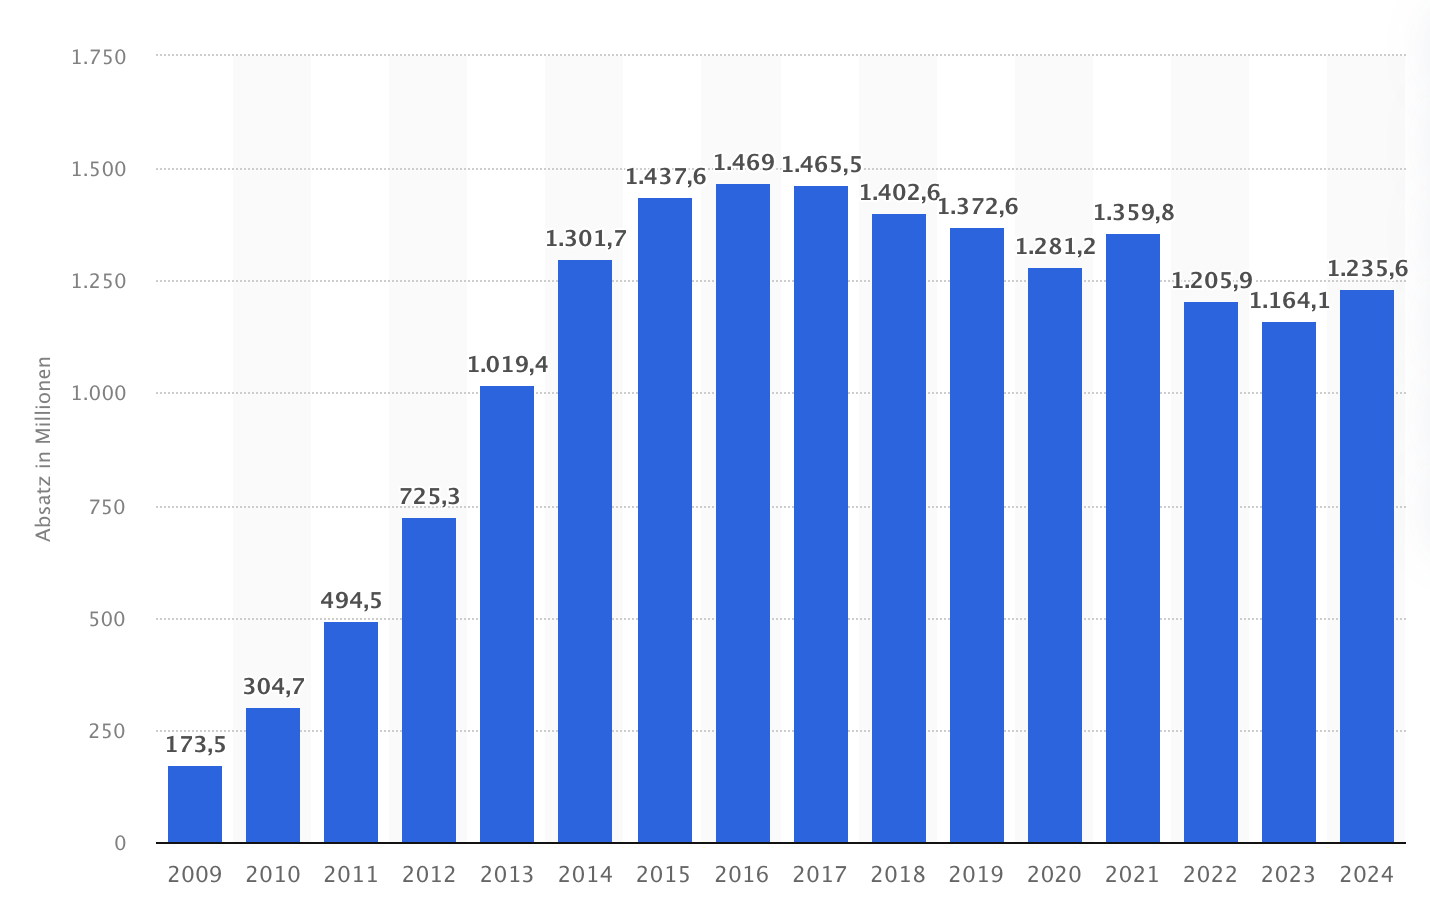
\includegraphics[width=0.90\textwidth]{img/Absatz von Smartphones.png}
    \caption{Absatz von Smartphones weltweit 2009 - 2024}
	\cite{statista_absatz_2025}
    \label{fig:absatz_smartphones}
\end{figure}

Neben der unmittelbaren Zugänglichkeit ermöglicht Mobile Learning auch die Integration von sensorischen Daten (z.B. GPS, Bewegungssensoren) für ortsbezogene oder kontextabhängige Lernangebote. Die Kombination von Mobilität, Interaktivität und individualisierbaren Lerninhalten macht Mobile Learning zu einem wichtigen Bestandteil moderner, digitaler Lernlandschaften, der die Entwicklung von E‑Learning nach MOOCs fortführt \parencite[S.~10]{sharples_theory_2010}.

\subsection{Microlearning \& Gamification}

Aufbauend auf den Möglichkeiten des Mobile Learning, das Lernen jederzeit und überall ermöglicht, entwickelte sich in den folgenden Jahren zunehmend der Trend zum Microlearning. Während Mobile Learning den technologischen Rahmen bereitstellt, stellt \textbf{Microlearning} ein darauf abgestimmtes didaktisches Konzept dar: Wissen wird in kurzen, modularisierten Lerneinheiten vermittelt, die oft nur wenige Minuten in Anspruch nehmen und sich flexibel in den Alltag integrieren lassen \parencites[S.~18--20]{hug_outline_2007}[S.~5--8]{buchem_microlearning_2010}. 

Parallel dazu gewann das Konzept der \textbf{Gamification} an Bedeutung. Obwohl dieses Konzept schon seit den 80er-Jahren im Marketing Anwendung findet, wurde es im Bildungsbereich wesentlich später relevant. Gamifizierung ist ein Ansatz, der spieltypische Elemente – wie Punkte, Abzeichen, Ranglisten oder Levels – auf nicht-spielerische Kontexte überträgt, um Motivation und Engagement der Lernenden zu fördern \parencite[S.~452]{schlag_gamifizierung_2021}. Ergänzend entwickelten sich \textit{Serious Games} bzw. \textit{Digital Game Based Learning}, die über die spielerische Form hinaus spezifische Lerninhalte vermitteln \parencite[S.~14]{niegemann_kompendium_2008}.

In diesem Zusammenhang etablierten sich auch zunehmend \textbf{adaptive Lernsysteme}, die durch Algorithmen den individuellen Wissensstand und Lernfortschritt berücksichtigen und Lerninhalte dynamisch anpassen. Durch die Kombination von Microlearning-Ansätzen mit Gamification-Elementen entstanden so hochgradig personalisierte Lernumgebungen, die Effizienz, Motivation und Flexibilität des Lernens gleichermaßen unterstützen \parencite[S.~1f]{katsaris_adaptive_2021}.

\subsection{Künstliche Intelligenz \& digitale Transformation des Lernens}

Ab Ende der 2010er-Jahre hielten erste \textbf{KI-gestützte Systeme} Einzug in das digitale Lernen. Chatbots wurden als virtuelle Tutoren eingesetzt, die Lernende bei Fragen unterstützen oder Feedback in Echtzeit bereitstellen. Ergänzend kamen Empfehlungssysteme zum Einsatz, die auf Grundlage des bisherigen Lernverhaltens individuelle Lernpfade vorschlagen \parencites[S.~1f]{harry_role_2023}[S.~42ff]{zhai_review_2021}.

Gleichzeitig wurden immersive Technologien wie Virtual, Augmented und Mixed Reality (VR/AR/MR) in Trainings- und Bildungskontexten erprobt, insbesondere in der Medizin, im technischen Training oder in simulationsbasierten Lernumgebunge \parencites[S.~3f]{rocha_bicalho_use_2023}[S.~251]{anatolevna_kastornova_international_2022}[S.~2f]{radianti_systematic_2020}. Gerade Simulatoren profitieren dabei von immersiven Umgebungen, die es erlauben, komplexe Handlungen realitätsnah, risikofrei und mit unmittelbarem Feedback zu erproben. Darüber hinaus gewann das Konzept des \textbf{Blended Learning~2.0} an Bedeutung, das über die bloße Kombination von Präsenz- und Online-Formaten hinausgeht und verstärkt auf adaptive Lernpfade, kollaborative Ansätze und digitale Partizipation setzt \parencites{seufert_schulleitertagung_2014}{news_aktuell_gmbh_e-learning_2025}.

Die COVID-19-Pandemie fungierte als entscheidender Beschleuniger der digitalen Bildung. Innerhalb kürzester Zeit waren Schulen, Hochschulen und Weiterbildungseinrichtungen gezwungen, ihre Lehrangebote vollständig auf Distanzformate umzustellen, sodass digitale Plattformen und Werkzeuge schlagartig zum zentralen Medium des Lehrens und Lernens wurden. Der Einsatz von Videokonferenz-Plattformen wie Zoom oder Microsoft Teams stieg rasant, während klassische Lernplattformen mit interaktiven Tools ergänzt wurden, um soziale Nähe trotz physischer Distanz herzustellen \parencite[S.~1f]{hodges_torrey_2020}. Der Fokus verlagerte sich in dieser Phase stark auf die \textbf{digitale Didaktik}: Interaktivität, soziale Eingebundenheit und lernförderliches Feedback wurden zu zentralen Kriterien für den Erfolg digitaler Bildungsangebote. Gerade im Bereich simulationsbasierten Lernens gewann die Möglichkeit, virtuelle Trainingsumgebungen auch remote zugänglich zu machen, zusätzlich an Bedeutung.

Mit dem Aufkommen generativer KI-Systeme wie ChatGPT, DALL·E oder Claude haben sich die Möglichkeiten im E-Learning grundlegend verändert. KI kann heute Lerninhalte automatisiert erstellen, personalisierte Tutorensysteme bereitstellen und individuelle Lernpfade in Echtzeit anpassen \parencite[S.~43]{zhai_chatgpt_2023}. Gleichzeitig verschiebt sich der Fokus von klassischen LMS zu \textbf{Learning Experience Platforms (LXP)}, die Lernenden eine kuratierte, KI-gestützte Auswahl an Inhalten bieten \parencite[S.~1]{cockrill_learning_2021}. Ergänzend entwickelt sich \textbf{Learning Analytics~2.0}: prädiktive Systeme identifizieren Lernprobleme frühzeitig und unterstützen Lehrende bei Interventionen \parencite[S.~1979f]{ifenthaler_utilising_2020}. Parallel dazu werden immersive Simulatoren zunehmend mit KI-Technologien verknüpft, die Szenarien dynamisch anpassen und Echtzeit-Feedback generieren können. Schließlich gewinnen \textbf{Microcredentials} und digitale Zertifikate an Bedeutung, um lebenslanges Lernen sichtbar und flexibel dokumentierbar zu machen \parencite[S.~1]{gish-lieberman_micro-credentials_2021}.

